% Blindleistungskompensation
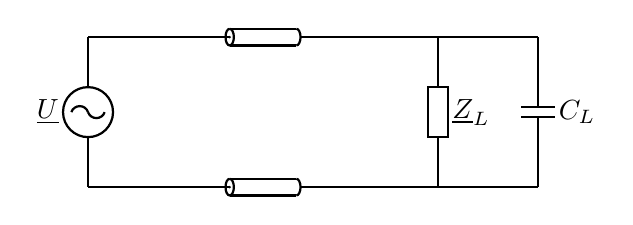
\begin{tikzpicture}[scale=2.54]%
% dpic version 2024.01.01 option -g for TikZ and PGF 1.01
\ifx\dpiclw\undefined\newdimen\dpiclw\fi
\global\def\dpicdraw{\draw[line width=\dpiclw]}
\global\def\dpicstop{;}
\dpiclw=0.8bp
\dpiclw=0.8bp
\dpicdraw (0,0)
 --(0,-0.25)\dpicstop
\dpicdraw (0,-0.375) circle (0.049213in)\dpicstop
\dpicdraw (-0,-0.375)
 ..controls (-0.005978,-0.357065) and (-0.022762,-0.344968)
 ..(-0.041667,-0.344968)
 ..controls (-0.060571,-0.344968) and (-0.077355,-0.357065)
 ..(-0.083333,-0.375)\dpicstop
\dpicdraw (0,-0.375)
 ..controls (0.005978,-0.392935) and (0.022762,-0.405032)
 ..(0.041667,-0.405032)
 ..controls (0.060571,-0.405032) and (0.077355,-0.392935)
 ..(0.083333,-0.375)\dpicstop
\dpicdraw (0,-0.5)
 --(0,-0.75)\dpicstop
\draw (-0.125,-0.375) node[left=-2bp]{$ \underline{U}$};
\dpicdraw (0,0)
 --(0.5,0)\dpicstop
\dpicdraw (1.0625,0)
 --(1.25,0)\dpicstop
\dpicdraw (0.5,0)
 --(0.708333,0)\dpicstop
\dpicdraw[line width=0.4bp](0.708333,0) circle (0.00109in)\dpicstop
\dpicdraw (0.708333,-0.041667)
 --(1.041667,-0.041667)\dpicstop
\dpicdraw (1.041667,-0.041667)
 ..controls (1.053173,-0.041667) and (1.0625,-0.023013)
 ..(1.0625,0)
 ..controls (1.0625,0.023013) and (1.053173,0.041667)
 ..(1.041667,0.041667)\dpicstop
\dpicdraw (1.041667,0.041667)
 --(0.708333,0.041667)\dpicstop
\dpicdraw (0.708333,0.041667)
 ..controls (0.696827,0.041667) and (0.6875,0.023013)
 ..(0.6875,0)
 ..controls (0.6875,-0.023013) and (0.696827,-0.041667)
 ..(0.708333,-0.041667)
 ..controls (0.71984,-0.041667) and (0.729167,-0.023013)
 ..(0.729167,0)
 ..controls (0.729167,0.023013) and (0.71984,0.041667)
 ..(0.708333,0.041667)\dpicstop
\dpicdraw (1.25,0)
 --(1.75,0)\dpicstop
\dpicdraw (1.75,0)
 --(1.75,-0.25)\dpicstop
\dpicdraw (1.75,-0.5)
 --(1.8,-0.5)
 --(1.8,-0.25)
 --(1.7,-0.25)
 --(1.7,-0.5)
 --(1.75,-0.5)\dpicstop
\dpicdraw (1.75,-0.5)
 --(1.75,-0.75)\dpicstop
\draw (1.8,-0.375) node[right=-2bp]{$ \underline{Z}_L$};
\dpicdraw (1.75,0)
 --(2.25,0)\dpicstop
\dpicdraw (2.25,0)
 --(2.25,-0.35)\dpicstop
\dpicdraw (2.166667,-0.35)
 --(2.333333,-0.35)\dpicstop
\dpicdraw (2.166667,-0.4)
 --(2.333333,-0.4)\dpicstop
\dpicdraw (2.25,-0.4)
 --(2.25,-0.75)\dpicstop
\draw (2.333333,-0.375) node[right=-2bp]{$ C_L$};
\dpicdraw (2.25,-0.75)
 --(1.75,-0.75)\dpicstop
\dpicdraw (0,-0.75)
 --(0.5,-0.75)\dpicstop
\dpicdraw (1.0625,-0.75)
 --(1.25,-0.75)\dpicstop
\dpicdraw (0.5,-0.75)
 --(0.708333,-0.75)\dpicstop
\dpicdraw[line width=0.4bp](0.708333,-0.75) circle (0.00109in)\dpicstop
\dpicdraw (0.708333,-0.791667)
 --(1.041667,-0.791667)\dpicstop
\dpicdraw (1.041667,-0.791667)
 ..controls (1.053173,-0.791667) and (1.0625,-0.773013)
 ..(1.0625,-0.75)
 ..controls (1.0625,-0.726988) and (1.053173,-0.708333)
 ..(1.041667,-0.708333)\dpicstop
\dpicdraw (1.041667,-0.708333)
 --(0.708333,-0.708333)\dpicstop
\dpicdraw (0.708333,-0.708333)
 ..controls (0.696827,-0.708333) and (0.6875,-0.726988)
 ..(0.6875,-0.75)
 ..controls (0.6875,-0.773013) and (0.696827,-0.791667)
 ..(0.708333,-0.791667)
 ..controls (0.71984,-0.791667) and (0.729167,-0.773013)
 ..(0.729167,-0.75)
 ..controls (0.729167,-0.726988) and (0.71984,-0.708333)
 ..(0.708333,-0.708333)\dpicstop
\dpicdraw (1.25,-0.75)
 --(1.75,-0.75)\dpicstop
\end{tikzpicture}%
